%!TEX root = ../master.tex
\chapter{Implementation}\label{ch:implementation}
Our development chapter. \todo{We describe Rear Infused Illumination, and add all theory we have on the things mention if RID - for example BLOBs, contrast, illumination and so on.}

\section{Rear Diffused Illumination} \label{sec:RDI}
\begin{figure}[!h]
\centering	\includegraphics[width=0.5\textwidth]{sketchAugmentedBoard}
\label{Fig:sketch} \caption{An sketch of our RDI table.}
\end{figure}
The interaction on the game board table will be based on rear diffused illumination as described in Multi-Touch Technologies \citep{multiTT}. This means, as shown in figure 6.1, that infrared (IR) lamps will be placed underneath the table's surface, projecting IR light upwards. A webcam below the table will be equipped with an IR filter obtained from a floppy disc, meaning it will primarily detect IR light. Furthermore, the table's surface, made of transparent material, needs a diffuser material just above or beneath it in order to diffuse the light. The purpose of this diffuser is to scatter the IR light and make objects hovering over the surface less visible to the camera. When an object touches the surface, the area of contact reflects more IR light than the untouched areas of the diffuser. This reflected light is captured by the camera, and can then be extracted as a BLOB.

Choosing such a solution has its advantages and disadvantages. First of all, there is no need for a compliant surface or soldering for an LED frame, since we are using a diffuser in order to reflect the IR-light coming from below. The illuminators for that can be bought ready to go, so there is no need to build them. A disadvantage comes from the RDI having difficulties with getting even illumination, since the IR-lights might not cover the table's surface completely, or they might overlap, causing areas with an excessive amount of refledcted IR light. This can result in false BLOBs, as well as BLOBs of lower contrast which are hard to detect. All this can challenge the software's detection of the desired BLOBs.

\section{Physical Design} 
\begin{figure} [!h]
\centering 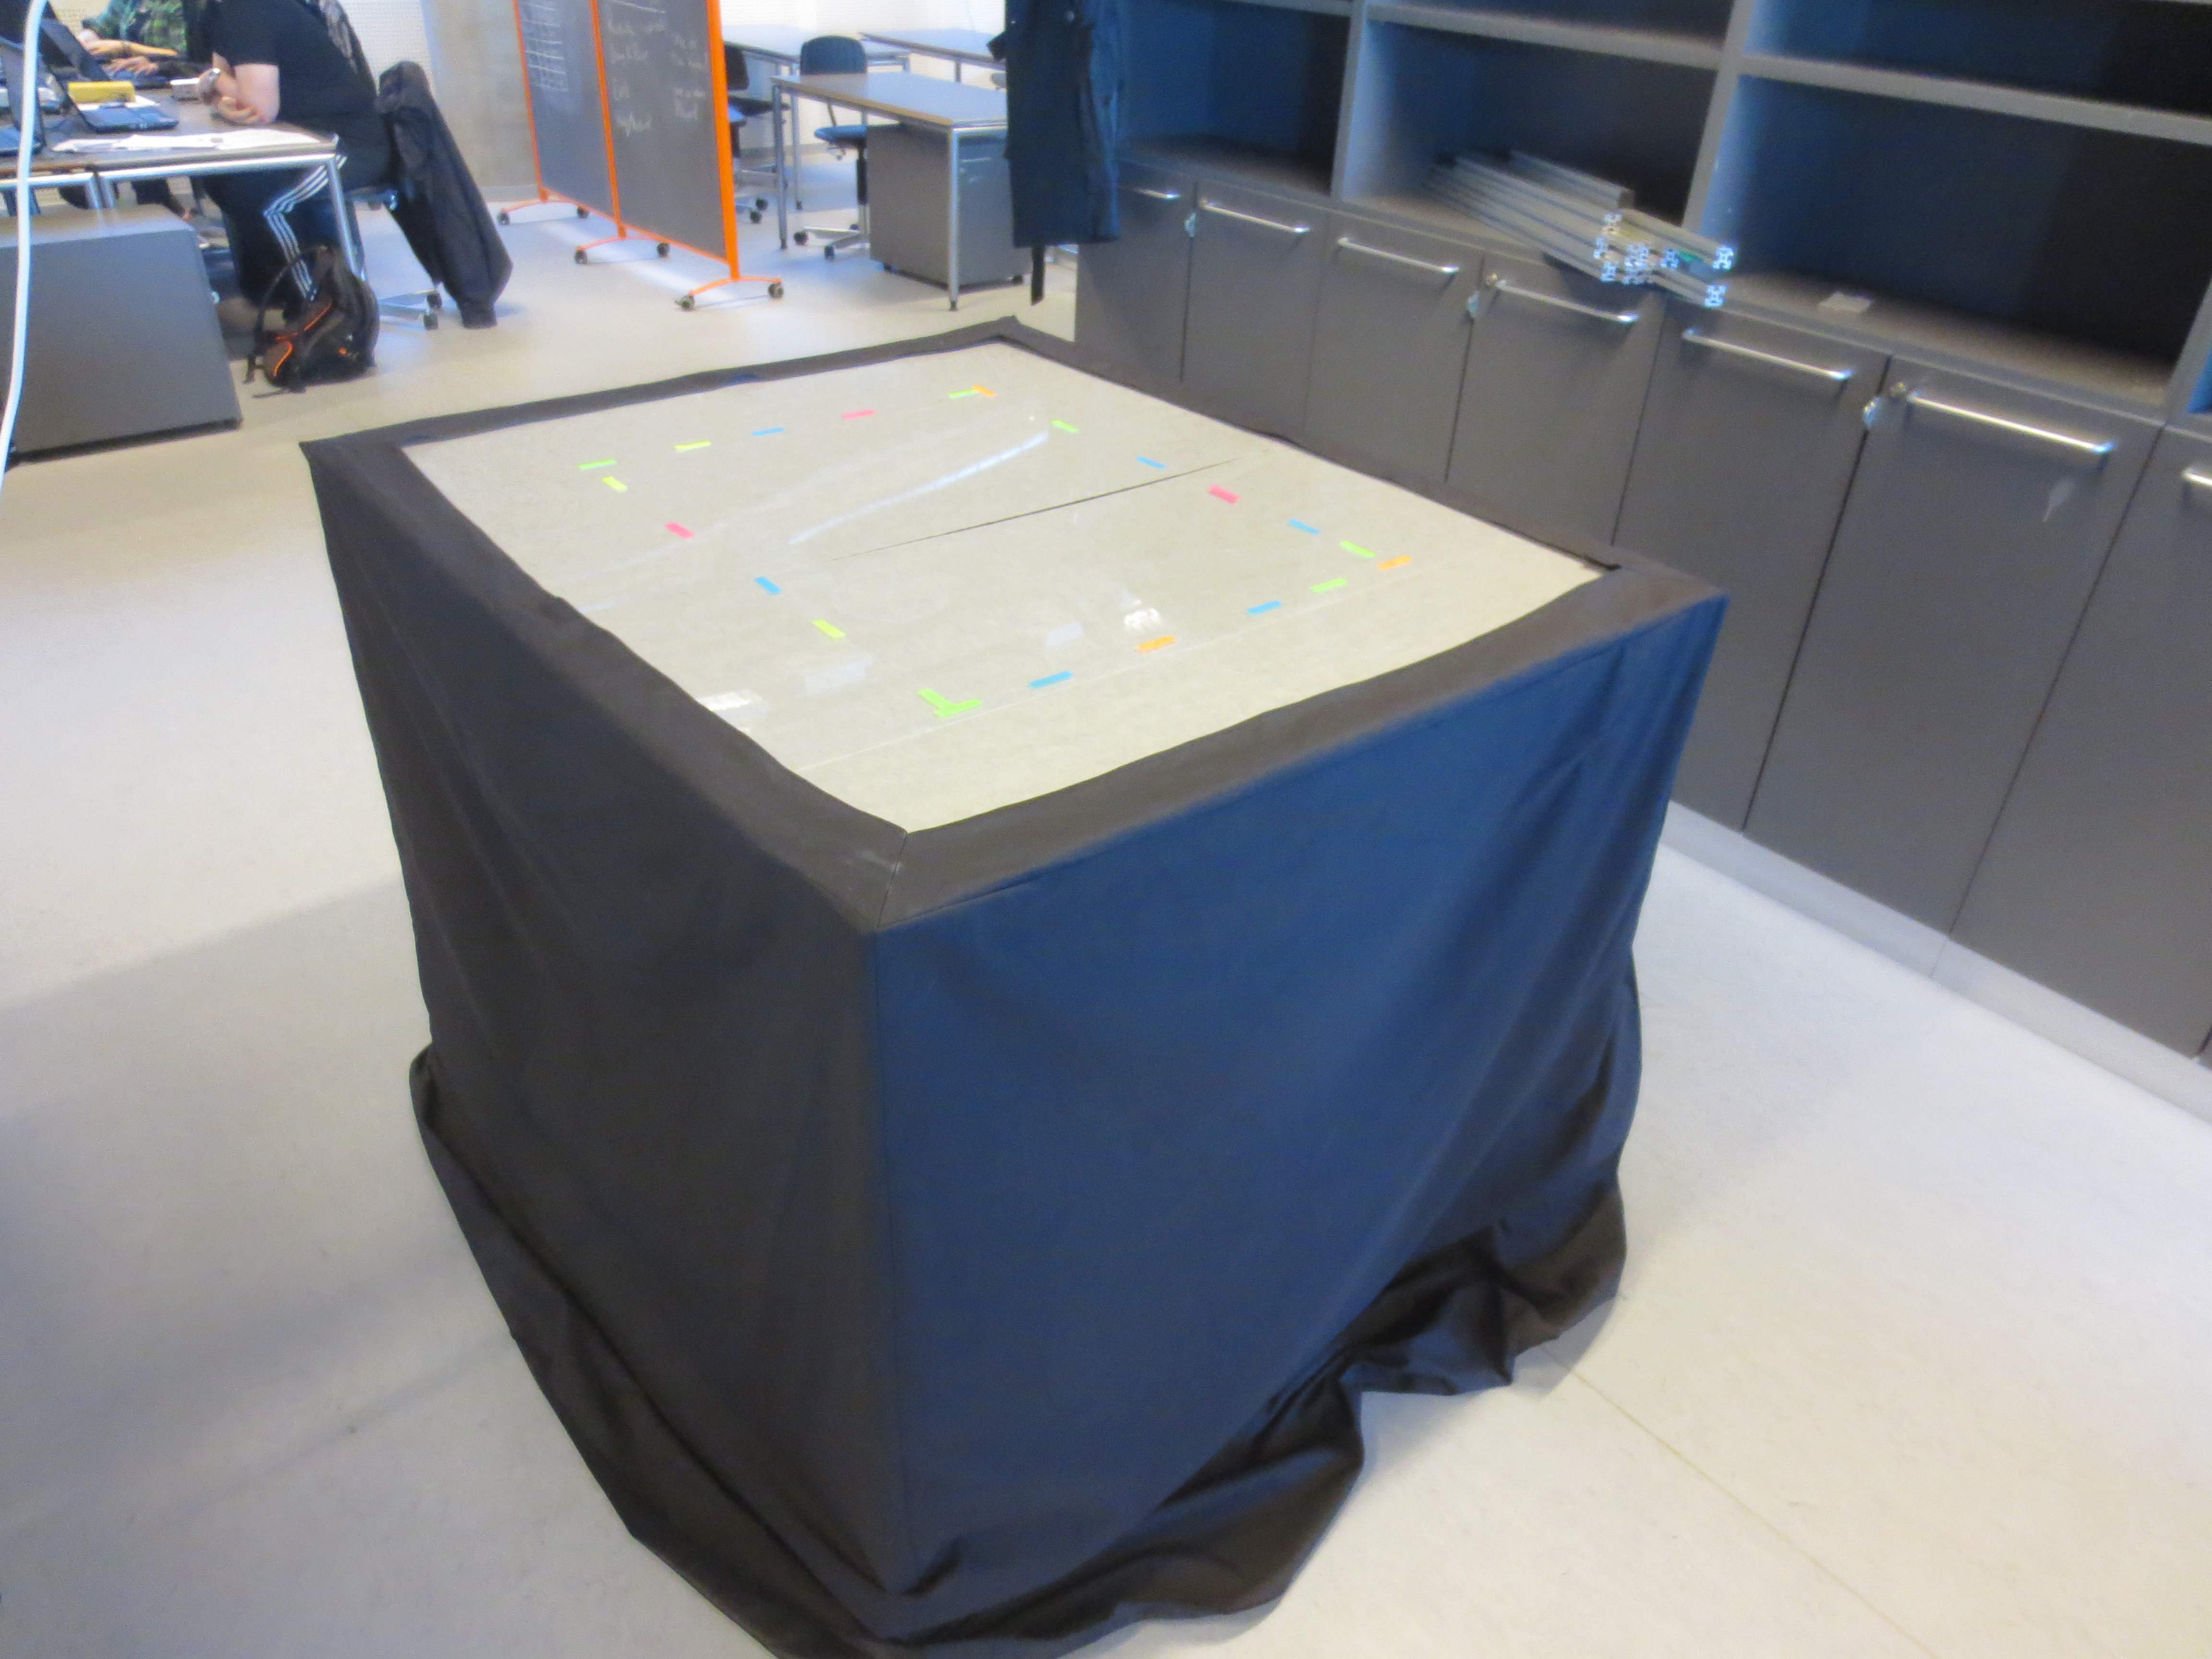
\includegraphics[width=0.5\textwidth]{Table}
\label{Fig:Table} \caption{The touch table}
\end{figure}
This section will describe the physical aspect of our product.
Our table's surface is made from acrylic glass, and below are four IR lamps, as well as a webcam with and IR filter, and a short-throw projector, which will project images on the table. The webcam and IR lamps are there to facilitate RDI, as explained in Section~\ref{sec:RDI}. All these elements are placed in a manner that spreads the IR light from the lamps as evenly as possible.

The outer frame of the table is constructed from 3 different lengths of aluminium rods, giving the table a final size of 120 x 102 x 89 cm.
In order to keep outside IR light from disturbing the image as much as possible, a black cloth is covering the table at the sides. The cloth has the additional benefit of making the projection from the short-throw projector clearer. 

As diffuser material, baking paper was chosen, as it is easily available. The paper is placed underneath the glass surface, as tight as possible, as placing it on top results in too much light being reflected by the acrylic glass into the webcam. When applying the diffuser, we encountered a problem: If the diffuser is not attached tight enough to the glass, touching the surface does not result in enough IR light being reflected. This was remedied by tightening the baking paper with duct tape.

\section{Image Processing}
To facilitate user interaction, a software module is needed to analyse a video input and recognize specific features and change in it over time. As described in Section~\ref{sec:ReqSpec}, there are two main criteria for this software's minimum implementation. It needs to:
\begin{itemize}
\item Recognise which gesture is done when selecting player.
\item Recognise when a tile is selected for terraforming.
\end{itemize}

To do these, BLOBs need to be extracted from the video input through segmentation. Since it is difficult to create a uniform surface of reflected IR-light, it might be necessary to apply background subtraction to the input before segmentation. Furthermore, since this is a video feed rather than a static image, changes in illumination may need to be accounted for as well by looping the background subtraction. This leads to a three-step solution for processing the video input:
\begin{enumerate}
\item Prepare video frame for segmentation (Pre-segmentation).
\item Segment image (Segmentation, includes denoising/smoothing).
\item Conditionally change data depending on the BLOB analysis
\end{enumerate}
Point 2 and 3 of the steps, are in a constant loop. Whenever one or more new BLOB(s) is analysed, the program conditionally changes data depending on that analysis. A new BLOB after that causes other changes and so on. The code should base the background subtraction on frames before the segmentation starts and use these as reference.

\subsection{Segmentation methods}
There are several methods for segmenting images. Relevant methods are discussed in this section. Since this project deals with video as opposed to static images, a single threshold with a fixed threshold value is not useful. As described in Section~\ref{sec:RDI}, the hardware setup uses RDI with IR light sources, and an  infrared filter on a web camera. This should create an ideal image for segmentation using an adaptive global thresholding method. This method makes use of the histogram of an image to identify the most optimal threshold value\citep{Moeslund2012c4}. In an ideal image, the histogram will have two distinct 'mountains' of pixel values, that is to say, there will be two groups of pixels that, within each group, have a similar brightness while at the same time the groups themselves are isolated from each other. In the case of this project, the image produced is expected to have bright spots where the board is touched, on a dark plane which is to be considered the background. The software then needs to identify an optimal threshold value between these two groups. One such method, is to evaluate the formula in Figure~\ref{eq:otsu} for each brightness value in the histogram. The result with the lowest value is then selected.\todo {Not sure we should be talking about otsu at all anymore, since we are not really using that.}
\begin{figure}[h]
	\begin{align*}
	C(T)&=M_1(T)\cdot\sigma_1^2(T)+M_2(T)\cdot\sigma_2^2(T)
	\end{align*}
	\caption{$M_1(T)$ is the number of pixels left of $T$ and $M_2(T)$ is the number of pixels to the right. $\sigma_1^2(T)$ and $\sigma_2^2(T)$ is the variance of the pixels to the left and right repsectively \label{eq:otsu} \citep[p. 61]{moeslund_introduction_2012_chapter_5}}
\end{figure}

\section{Rendering of game board}
\begin{figure}[h!]
\centering 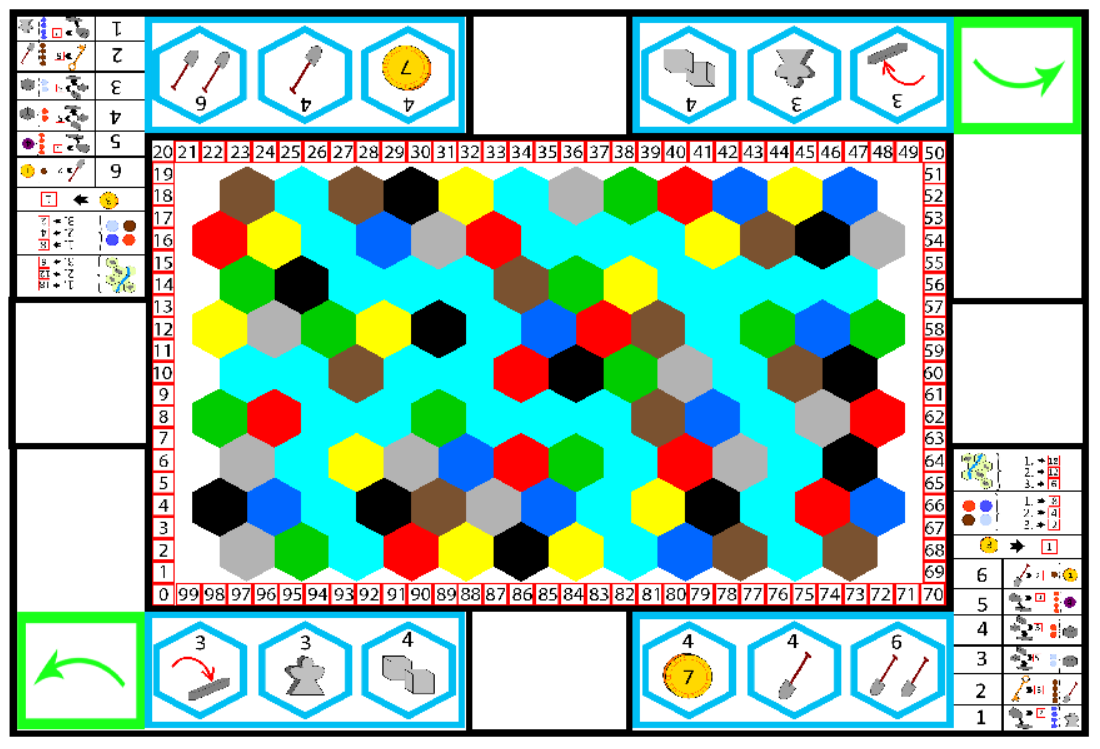
\includegraphics[width=0.5\textwidth]{BoardWithTiles}
\caption{The game board \label{Fig:Board}}
\end{figure}\todo{Kill these undo buttons, make them die die DIE}
In order for the program to be able to change the game tiles through terraforming, it must have access to them from the start. This is done, by having the program render out all the tiles. The border around the actual tiles are made from a background image, which is imported as is. This image contains the outline of a player area for each player, the point counter, and the border for each exclusive action. 
\begin{figure}[h!]
\centering 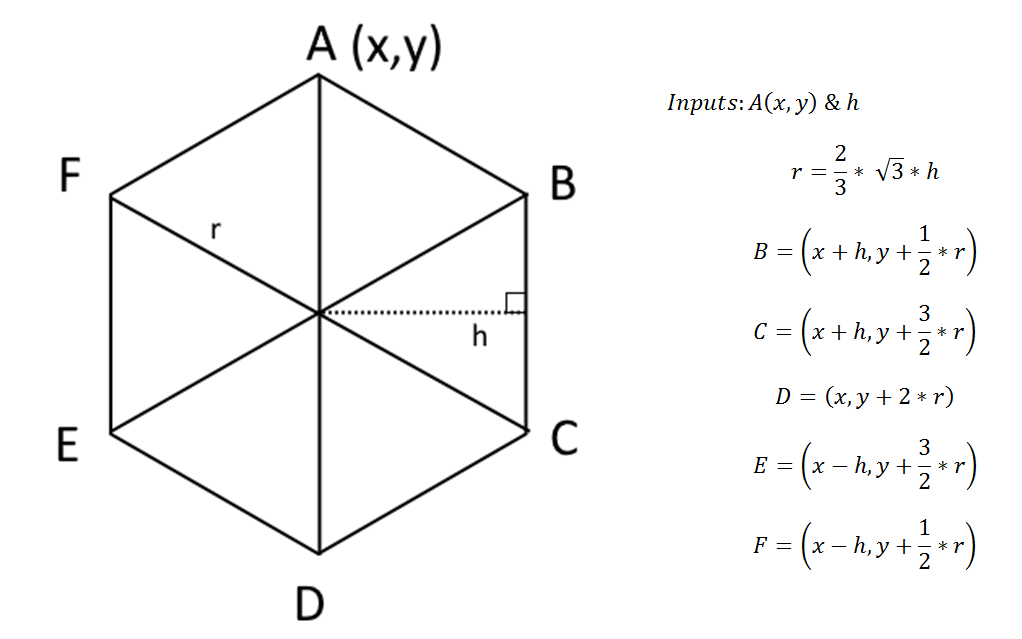
\includegraphics[width=0.7\textwidth]{HexWithMath}
\caption{Relations between height and points in hexagon \label{Fig:HexWithMath}}
\end{figure}\todo{}

On top of this image is the rendering of the tiles themselves. This is done with a function, which takes a two-dimensional coordinate, the height of the hexagon, the image on which to draw on, and a colour as parameters. The function calculates the radius based on the height input, which is then used to calculate the relations between the coordinate input and the remaining coordinates. Then the function fills it with the given colour. The equations used to calculate the points in the hexagon are shown in Figure \ref{Fig:HexWithMath}.

With this method, the program renders out the board row by row, saving the coordinate for the A-point of each tile and the colour in two different arrays. The resulting rendered board is what is shown in Figure \ref{Fig:Board}.
